\chapter{Approximation Algorithms for Maximum CMO}
\label{approximation}

This chapter reviews the approximation algorithms for solving the maximum CMO problem. To begin with, \citet{goip99} represent the problem as a graph theoretic abstraction and prove the NP-hardness of the problem. The authors further propose a special class of CMO problem for which 3-approximation algorithm runs in $O(n^6)$ time. In the next few sections, the 6-approximation algorithm with better time complexity for the same class of problems, as proposed in \citet{agmw07}, is discussed. Moreover, an $O(\sqrt n)$ approximation algorithm, also suggested by \citet{agmw07}, for the 3-dimensional self-avoiding walk is summarized. Such results are the first of their kind for 3-dimensional self-avoiding walk.

%\section{NP-hardness and Approximation Result for Special Cases}
\section {CMO as a Graph Theoretic Optimization Problem}
Let $Z$ be an integer grid in $\mathbb{R}^2$ or $\mathbb{R}^3$. A \emph{self-avoiding walk} is a one-to-one mapping $f:V =\{v_1,v_2,....,v_n\}\rightarrow Z$ such that $\|v_i - v_{(i+1)}\| = 1$ and $v_i \ne v_j$, $1 \leq (i,j) \leq n$. Self-avoiding walks are used to represent protein structures as physical evidences show that proteins cannot be represented by arbitrary edges.

A {\it contact map} is an ordered graph $G = (V,E)$ where $V = \{v_1,v_2,....,v_n\}$ is the set of vertices and $E = \{(v_i, v_j): \|j-i\| >1 \text{ and } \|v_i - v_j\| =1\}$ is the set of edges. Contact maps are useful representation of proteins where each vertex represents one amino acid and the edges are the proxy for the pairs of amino acids (not in the linear sequence) whose centroids are closer than a fixed threshold. Fig. \ref{fig:A self-avoiding walk} and \ref{fig:A contact Map Example} show the examples of a self-avoiding walk and its corresponding contact map.

Given two contact maps $G_1=(V_1,E_1)$ and $G_2=(V_2,E_2)$ where $V_1=\{v_1,v_2,\cdots,v_{n_1}\}$ and $V_2=\{u_1,u_2,\cdots,u_{n_2}\}$, $n_1$ and $n_2$ being the total number of vertices in $V_1$ and $V_2$ and two subsets $S_1 \subseteq \{v_1,v_2,\cdots,v_{n_1}\}$ and $S_2 \subseteq \{u_1,u_2,\cdots,u_{n_2}\}$ with $|S_1| = |S_2|$, the \emph{contact map overlap} is defined as the maximum cardinality of the set $|\{(v_i,v_j) \in E_1 : v_i,v_j \in S_1, (f(v_i), f(v_j)) \in E_2|$ under some {\it order-preserving bijection} $f$. Fig. \ref{fig:A contact Map overlap Example} explains a contact map overlap between the two graphs. 

\section{NP-Hardness of CMO}
The contact map overlap problem, in its graph theoretical representation, is NP-hard. This implies that it is less probable that a polynomial time algorithm exists that computes the contact map overlap between two graphs of self-avoiding walks.

The structure of the proof is suggested in \citet{goip99}. The proof of the above is deduced with the help of two other lemmata. In the first step, it is proved that computation of the overlap of two $2$-stack graphs which have a maximum degree $3$ is NP-hard. The reduction is from the Planar $3$-SAT problem which is known to be NP-complete itself \citep{lich82}. Let the Planar $3$-SAT problem instance consist of $n$ variables $\{x_1,x_2,\cdots,x_n\}$ and $m$ clauses $\{c_1,c_2,\cdots,c_m\}$. This instance of the problem is mapped into two $2$-stack graphs $G_1$ and $G_2$. These two graphs contain variable and clause gadgets arranged in a linear layout according to a planar embedding of the formula. Between each variable and clause gadgets (nodes in the graph), enforcing gadgets are inserted which consist of $5m$ (on $10m$ nodes) edges. Once the two graphs are constructed, the constraints of the Planar $3$-SAT formula is satisfied by an order preserving bijection between the vertices of $G_1$ and $G_2$. The order-preserving bijection is as follows. The variable node in each variable gadget of $G_1$is mapped to the true literal node in the corresponding variable gadget of $G_2$. Further, nodes in the enforcing gadgets of $G_1$ are mapped to nodes in the corresponding gadget of $G_2$. Finally, the clause node in each clause gadget of $G_1$ is mapped to a true literal node in the corresponding clause gadget of $G_2$. The two graphs can thus be reduced to an instance of the Planar $3$-SAT problem and since the Planar $3$-SAT problem is NP-complete, it is NP-hard to compute the overlap of the two 2-stack graphs of maximum degree $3$.

The second step involves proving that it is also NP-hard to compute the overlap of two 2-stack graphs which have a maximum degree $1$. The proof follows similar argument, \emph{i.e.} the problem again is reduced to a Planar $3$-SAT problem in polynomial time. The only difference is the way in which the two graphs are constructed such that they are easily decomposable into two stacks each having degree $1$. The order-preserving bijection follows the same rules.

These two proofs are successfully used to construct the proof of NP-hardness of the computation of the contact overlap of two self-avoiding walks. The structure of the proof is very similar, the only difference being the enforcing gadgets used for the construction of the Planar $3$-SAT Problem. 

\section{Polynomial Algorithm for Stack, Queue and Staircase}
Since finding the contact map overlap between two self-avoiding walks is NP-hard, \citet{goip99} propose ways to decompose these graphs into simpler special cases and derived polynomial time algorithms for these special cases. Before understanding these special cases, it is necessary to understand three different types of relations between pairs of edges in a contact map.
\begin{noindlist}
\item {\it Disjoint Edges:}  Let $e_1 = (v_i, v_j)$ and $e_2 = (v_{i^{\prime}}, v_{j^{\prime}})$ be two
edges in $G$. Then $e_1$ and $e_2$ are \emph{disjoint} if $(i,j) \cap (i^{\prime},j^{\prime}) = \emptyset$.
\item {\it Containing Edges:} $e_1$ \emph{contains} $e_2$ if  $(i,j) \supset (i^{\prime},j^{\prime})$.
\item {\it Overlapping Edges:} Two edges $e_1$ and $e_2$ \emph{overlap} each other if $(i,j) \cap (i^{\prime},j^{\prime}) \neq \emptyset$ and one edge does not contain the other (unless an end point is shared).
\end{noindlist}

\begin{figure}[htbp]
\begin{minipage}[b]{0.33\linewidth}
\centering
 
\centering
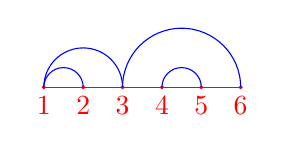
\begin{tikzpicture}[scale=0.5]


\foreach \i in {1,...,5} {
        \draw[red] (\i,1) -- (\i + 1,1)node[pos=0.0,below] {\i};
        \filldraw[red] (\i,1) circle (1pt);


 }

\draw[red] (6,1) -- (5,1)node[pos=0.0,below] {6};
\filldraw[red] (6,1) circle (1pt); 



\draw[blue, thin] (1,1) arc(180:0:0.5); 
\draw[blue, thin] (1,1) arc(180:0:1); 
\draw[blue, thin] (3,1) arc(180:0:1.5);
\draw[blue, thin] (4,1) arc(180:0:0.5);
\end{tikzpicture} 
 \vspace{0.65cm}
 \caption{Stack}
 \label{fig:Stack1}
\end{minipage}
\begin{minipage}[b]{0.33\linewidth}
\centering
 \input{queue}
 \vspace{0.65cm}
 \caption{Queue}
 \label{fig:Queue}
\end{minipage}
\begin{minipage}[b]{0.33\linewidth}
\centering
 \input{staircase}
 \vspace{0.65cm}
 \caption{Staircase}
 \label{fig:Staircase}
\end{minipage}
\end{figure}

Based on the above relations, \citet{goip99} propose three simpler graphs as follows:
\begin{noindlist}
\item {\it Stack:} A stack is defined as the contact map $(V,E)$ where if $e_1$ and $e_2$ are two edges in the contact map then either they contain one another, are disjoint or overlap at one end point.
\item {\it Queue:} A queue is defined as the contact map $(V,E)$ where if $e_1$ and $e_2$ are two edges in the contact map then they do not contain one another unless they share one end-point.
\item {\it Staircase:} A staircase is a special case of queue in which there are sets of mutually overlapping intervals such that either no two intervals in the different sets meet, or at most two of them overlap at an end-point.
\end{noindlist}
These graphs are illustrated in Figs. \ref{fig:Stack1}, \ref{fig:Queue} and \ref{fig:Staircase}. The proofs corresponding to the computation of contact map overlap for all of these special cases have similar structure and use dynamic programming. Some noteworthy results are presented in the following sections.

\subsection{$O(n^4)$ algorithm for maximum CMO of $2$-stack and degree-$2$ contact map}

Let $\text{co}(G_1,G_2)$ denote the overlap between $G_1$, a degree-2 stack of $n_1$ vertices and $G_2$, a degree-2 contact map of $n_2$ vertices. Now, since it is tabulated using dynamic programming, the subproblems are formed by computing the contact overlap of subgraphs like ${G_1}_{(v_a,v_b)}$ and ${G_2}_{(u_c,u_d)}$ where $v_1 \leq v_a < v_b \leq v_{n_1}$ and $1 \leq u_c < u_d \leq u_{n_2}$. There are few rules that are followed for computing the contact overlap of these two subgraphs recursively. The first one is that if two edges meet $v_b$(or $u_d$) then one must omit the lower first coordinate in each case. These are denoted by ${G_1}_{\hat{(v_a,v_b)}}$ or ${G_2}_{\hat{(u_c,u_d)}}$. Another rule is that an edge with the lowest end-point in one graph is mapped to the edge with the lowest endpoint in the other. These graphs can be denoted as $\text{co}({G_1}_{(v_a,v_b)}, {G_2}_{(u_c,u_d)})^l$. Similarly, edges with the highest end point will be mapped to one another. These graphs are denoted as $\text{co}({G_1}_{(v_a,v_b)}, {G_2}_{(u_c,u_d)})^h$. If both the edges are mapped, then the graph is denoted by $\text{co}({G_1}_{(v_a,v_b)}, {G_2}_{(u_c,u_d)})^{lh}$. The optimum contact map can be computed as follows:
\begin{eqnarray}
\label{sqs1}
\text{co}(G_1,G_2) = \max\{\text{co}({G_1}_{(v_1,v_{n_1})}, {G_2}_{(u_1,u_{n_2})})^h,\text{co}({G_1}_{\hat{(v_1,v_{n_1})}}, {G_2}_{(u_1,u_{n_2})})^h,\text{co}({G_1}_{(v_1,v_{n_1})}, \cap \nonumber \\ {G_2}_{\hat{(u_1,u_{n_2})}})^h,\text{co}({G_1}_{\hat{(v_1,v_{n_1})}}, {G_2}_{\hat{(u_1,u_{n_2})}})^h,\text{co}({G_1}_{(v_1,v_{(n_1-1)})}, {G_2}_{(u_1,u_{n_2})}),\text{co}({G_1}_{(v_1,v_{n_1})}, {G_2}_{(u_1,u_{(n_2-1)})}\}
\end{eqnarray}

\begin{figure}[htbp]
\begin{minipage}[b]{0.50\linewidth}
\centering
 
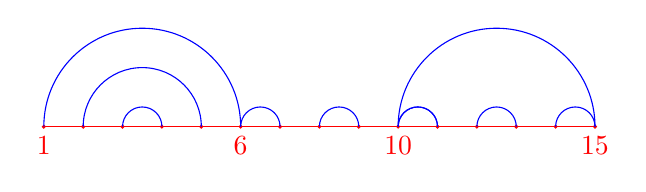
\begin{tikzpicture}[scale=0.5]
\centering
\label{staircasedecompisition}

\foreach \i in {1,...,14} {
        \draw[red] (\i,1) -- (\i + 1,1);
        \filldraw[red] (\i,1) circle (1pt);
 }
\draw[red] (15,1) -- (14,1)node[pos=0.0,below] {15};
\draw[red] (10,1) -- (9,1)node[pos=0.0,below] {10};
\draw[red] (6,1) -- (5,1)node[pos=0.0,below] {6};
\draw[red] (1,1) -- (2,1)node[pos=0.0,below] {1};
\filldraw[red] (15,1) circle (1pt);

\draw[blue, thin] (1,1) arc(180:0:2.5);
\draw[blue, thin] (2,1) arc(180:0:1.5);
\draw[blue, thin] (3,1) arc(180:0:0.5);
\draw[blue, thin] (6,1) arc(180:0:0.5);
\draw[blue, thin] (8,1) arc(180:0:0.5);
\draw[blue, thin] (10,1) arc(180:0:2.5);
\draw[blue, thin] (10,1) arc(180:0:0.5);
\draw[blue, thin] (10,1) arc(180:0:0.5);
\draw[blue, thin] (12,1) arc(180:0:0.5);
\draw[blue, thin] (14,1) arc(180:0:0.5);

\end{tikzpicture}
 \vspace{0.65cm}
 \caption{${G_1}_{(1,15)}$}
 \label{fig:$S_{(1,15)}$}
\end{minipage}
\begin{minipage}[b]{0.50\linewidth}
\centering
 
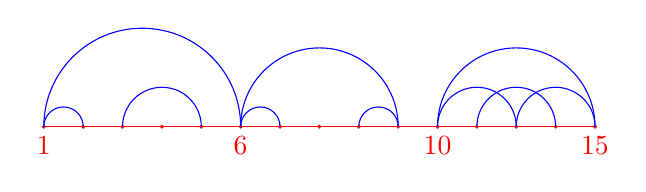
\begin{tikzpicture}[scale=0.5]
\centering
\label{staircasedecompisition}

\foreach \i in {1,...,14} {
        \draw[red] (\i,1) -- (\i + 1,1);
        \filldraw[red] (\i,1) circle (1pt);
 }
\draw[red] (15,1) -- (14,1)node[pos=0.0,below] {15};
\draw[red] (11,1) -- (10,1)node[pos=0.0,below] {10};
\draw[red] (6,1) -- (5,1)node[pos=0.0,below] {6};
\draw[red] (1,1) -- (2,1)node[pos=0.0,below] {1};
\filldraw[red] (15,1) circle (1pt);

\draw[blue, thin] (1,1) arc(180:0:2.5);
\draw[blue, thin] (1,1) arc(180:0:0.5);
\draw[blue, thin] (3,1) arc(180:0:1);
\draw[blue, thin] (6,1) arc(180:0:2);
\draw[blue, thin] (6,1) arc(180:0:0.5);
\draw[blue, thin] (9,1) arc(180:0:0.5);
\draw[blue, thin] (11,1) arc(180:0:2);
\draw[blue, thin] (11,1) arc(180:0:1);
\draw[blue, thin] (13,1) arc(180:0:1);
\draw[blue, thin] (12,1) arc(180:0:1);


\end{tikzpicture}
 \vspace{0.65cm}
 \caption{${G_2}_{(1,15)}$}
 \label{fig:$G_{(1,15)}$}
\end{minipage}
\end{figure}

Let us consider two subgraphs in Figs. \ref{fig:$S_{(1,15)}$} and \ref{fig:$G_{(1,15)}$}. Recursively,
the contact map of the two are given as:
\begin{eqnarray}
\label{sqs2}
\text{co}({G_1}_{(1,15)}, {G_2}_{(1,15)})^{lh} = 2+ \text{co}({G_1}_{(2,5)}, {G_2}_{(2,5)}) + \max\{\text{co}({G_1}_{(6,10)}, {G_2}_{(6,11)})^l,\text{co}({G_1}_{(7,10)}, {G_2}_{(7,11)})\} \cap \nonumber \\
+ \max \{\text{co}({G_1}_{(10,14)}, {G_2}_{(11,14)})^l,\text{co}({G_1}_{(11,15)}, {G_2}_{(12,15)})^h,\text{co}({G_1}_{(11,14)}, {G_2}_{(12,14)})\}
\end{eqnarray}
Here, one can see that node $1$ and node $15$ of each graph are matched for which $2$ is already counted in the calculation. The remaining calculation is for the intermediate edges. One subproblem in such setting is calculation of the number of matchings between nodes $2$ and $5$ of each graph. The next part of the equation computes the number of edges matching between node $6$ and $10$ in graph ${G_1}_{(1,15)}$ and $6$ and $11$ in graph ${G_2}_{(1,15)}$. It would take the maximum number of edges matched in two scenarios - one would be if the edge with lowest end-point at node $6$ matches with the lowest end point at node $6$ and the other would be to calculate the total number of edges matched from node $7$ to node $10$ in one and from node $7$ to node $11$ in the other. Matching at node $10$ and $11$ is excluded because there are no incoming edges at them. The third part of the calculation also follows the same order.

If $G_1$ is of size n, then from Eq. \ref{sqs1}, it can be seen that the total number of entries in the table is $O(n^4)$ and each table entry takes $O(1)$ time to compute. So the total time taken to compute all the entries is $O(n^4)$.

\subsection{$O(n^3)$ algorithm for maximum CMO of $2$-staircase and degree-$2$ contact map}

Considering $G_1$ to be a degree-2 staircase containing $n_1$ vertices and $G_2$ to be any degree-2 graph containing $n_2$ vertices, the computation of $\text{co}(G_1,G_2)$ is done again using a dynamic programming method. Firstly, the edges in $G_1$ and $G_2$ are numbered according to the ascending order of their right end points. If there are two edges which share the same right end point, the edge with the higher lowest end point is given higher number. A table is constructed with these two graphs having these $3$ indices - an edge $e_i$ from $G_1$, an edge $f_j$ from $G_2$ and the next entry is either a blank denoted by ``-" or contains a higher edge $f_{j^\prime}$ of $G_2$ whose interval overlaps edge $f_j$ at more than one points. Thus the table entries contain a contact overlap between a subgraph of $G_1$ denoted by ${G_1}_{e_i}$ which consists of all edges smaller than or equal to $e_i$ and a subgraph of $G_2$ denoted by ${G_2}_{(f_j,{f_{j^\prime}})}$ which consists of all edges smaller than or equal to $f_j$. There is a constraint of the above contact map which states that all edges of ${G_2}_{(f_j,{f_{j^\prime}})}$ that overlap $f_j$ also overlaps $f_{j^\prime}$ at more than one point. It is reasonable to say now that $f_{j^\prime}$ being the edge which overlaps $f_j$ at more than one point also matches an edge overlapping $e_i$. Also like the proof in the earlier case, if the highest endpoints of $e_i$ and $f_j$ map to each other, the corresponding contact map overlap is denoted by $\text{co}({G_1}_{e_i}, {G_2}_{(f_j,{f_{j^\prime}})})^h$.

Assuming that $G_1$ and $G_2$ contain $n_1$ and $n_2$ number of edges, the contact overlap between the two graphs is given by:
\begin{eqnarray}
\label{sqs3}
\text{co}(G_1,G_2) = \max\{\text{co}({G_1}_{n_1}, {G_2}_{({n_2},-)})^h, \text{co}({G_1}_{({n_1}-1)}, {G_2}_{({n_2},-)}),\text{co}({G_1}_{n_1}, {G_2}_{({n_2}-1,-)})\}
\end{eqnarray}
The subproblem $\text{co}({G_1}_{n_{e_1}}, {G_2}_{({n_{e_2}},-)})^h$ here which would recursively operate is also calculated similarly to the ones in the previous algorithm. The edges would be selected as those edges which overlap $e_i$ or $f_j$(in the staircase it would always be $e_({i-1})$) and the third entry would either be absent or would be the edge that overlaps $e_i$ or $f_j^\prime$ at more than one point. Now, considering all the columns in the table entries, the total number of entries are $O(n^3)$(if n is the number of vertices in $G_1$) and each table entry takes $O(1)$ time to compute. So the total time taken to compute all the entries is $O(n^3)$.

Now, any RNA structure (except one) is known to be decomposable into two degree-1 stacks \citep{goip99}. Any of these degree-1 stacks will have half of the edges that must be in the optimal alignment. So when this contact map of the RNA structure is optimized with any other contact map using the algorithm used for stack it can be guaranteed that the output will have at least half of edges mapped in the optimal solution. Thus one obtains a 2-approximation algorithm for constructing a contact map between two RNA structures. In the case of a queue, finding the contact map overlap between a queue and another contact map is NP-complete.  The approximation algorithm for queues are not shown separately because each queue can be decomposed into two staircases and following the same logic described above, there is a 2-approximation algorithm for computing the contact map overlap of a queue and another contact map.

The best results for approximation algorithm are obtained for a special case of contact map called augmented staircase. An \emph{augmented staircase} is a contact map which can be decomposed into a staircase and a stack with the constraint that for every stack edge and for every staircase edge, the interval formed by the edges are disjoint, overlap at an end point or the interval formed by the staircase edge contains the interval formed by the stack edge. The best polynomial results were obtained by computing the contact overlap between an augmented staircase and any degree-2 contact map.

\subsection{$O(n^6)$ algorithm for maximum CMO of augmented $2$-staircase and degree-$2$ contact map}

This algorithm builds the same way as the staircase algorithm and uses the stack algorithm as a subroutine. Let $G_1$ be a degree-2 augmented staircase of $n_1$ vertices and $G_2$ any degree-2 graph of $n_2$ vertices. Here edges in $G_1$ and $G_2$ are numbered according to ascending order of their right end points. $G_1$ can be decomposed into a staircase $T$ and a stack $S$. The stack algorithm is used to compute the table entries for the comparison between subgraphs of $S$ and subgraphs of $G_2$. In $T$, if two edges share the same right end-point, the edge with the higher left end point is numbered higher. The table here has four entries: $e=(v_i,v_j)$ from $T$, $f=(u_k,u_l)$ from $G_2$. The other two table entries are either empty or a higher edge $e^\prime$ of $T$ which overlaps with $e$ at more than one point and an edge $f^\prime$ of $G_2$ whose interval overlaps with $f$ at more than one point. The above table entry contains the constrained contact overlap between the subgraph $G_1$ denoted ${G_1}_{(e,{e^\prime})}$, consisting of all the edges less than or equal to $e$ and excluding the edges in $S$ which are in the interval formed by $e$ and $e^\prime$, and subgraph of $G_2$ denoted by ${G_2}_{(f,{f^\prime})}$, consisting of all edges less than or equal to $f$. Here  the constraint is that $e$ must map to $f$ and the mapped edges of ${G_2}_{(f,{f^\prime})}$ which overlap $f$ overlaps $f^\prime$ at more than a point. The contact overlap of $G_1$ and $G_2$ is thus given by:
\begin{eqnarray}
\label{sqs4}
\text{co}(G_1,G_2) = \max\{\text{co}(S,G),\max_{e \in T, f \in G_2}\{\text{co}({G_1}_{(e,-)} {G_2}_{(f,-)}) + s(j,l)\}.
\end{eqnarray}
\begin{eqnarray}
where, s(j,l) = \begin{cases}
    \max\{co(S_{(j,n_1)},{G_2}_{(l,{n_2})})^l,co(S_{(j+1,n_1)},{G_2}_{(l+1,n_2)})\}, & \\ \text{edges of $S$ and $G_2$ meet $j$, $l$ as left end points}.\\
    co(S_{(j+1,n_1),{G_2}_{(l+1,n_2)}}), \text{otherwise}.
  \end{cases}
\end{eqnarray}
The optimal bijection maps the highest edges of $T$ to an edge of $G_2$ or there is no such edge. The recursion maps the next highest edge in the subgraph of $T$ to $G_2$. So, if $G_1$is of size n, the total number of table entries is $O(n^4)$ and each entry takes $O(n^2)$ time to compute. Hence, the total time to compute the contact overlap between an augmented staircase and any degree-2 graph is $O(n^6)$. 

\section{Decomposition Theorem and Approximation Results}
In the earlier section, polynomial algorithms were proposed to calculate the maximum contact overlap between the special cases of graphs. In this section, it will be explored how any self-avoiding walk can be decomposed into these simpler graphs thereby facilitating the construction of contact maps for any self-avoiding walk. The first result, explained below, states that any self avoiding walk can be decomposed into two stacks and one queue.


\begin{figure}[htbp]
\begin{minipage}[b]{0.45\linewidth}
 \centering
 \newcommand*{\xMin}{0}%
\newcommand*{\xMax}{6}%
\newcommand*{\yMin}{0}%
\newcommand*{\yMax}{6}%

\newcommand*{\xshift}{0.20}%
\newcommand*{\yshift}{-0.20}%

\centering
\begin{tikzpicture}[scale=1.00]
% grid
    \foreach \i in {\xMin,...,\xMax} {
        \draw [very thin,gray] (\i,\yMin) -- (\i,\yMax)  node [below] at (\i,\yMin) {};
    }
    \foreach \i in {\yMin,...,\yMax} {
        \draw [very thin,gray] (\xMin,\i) -- (\xMax,\i) node [left] at (\xMin,\i) {};
    }

% start and end of the self avoiding walk
\filldraw[red] (2,3) circle (1pt);
\filldraw[red] (4,5) circle (1pt);

% self avoiding walk
\draw[red, ultra thick] (2,3) -- (2,2) -- (2,1) -- (1,1) -- (1,2) -- (1,3) -- (1,4) -- (2,4) --
(3,4) -- (3,3) -- (4,3) -- (4,2) -- (3,2) -- (3,1) -- (4,1) -- (5,1) -- (5,2) -- (5,3) --
(5,4) -- (4,4) -- (4,5);

% self avoiding walk indexing
\node (A) at (2+\xshift,3+\yshift) {1};
\node (B) at (2+\xshift,2+\yshift) {2};
\node (C) at (2+\xshift,1+\yshift) {3};
\node (D) at (1+\xshift,1+\yshift) {4};
\node (E) at (1+\xshift,2+\yshift) {5};
\node (F) at (1+\xshift,3+\yshift) {6};
\node (G) at (1+\xshift,4+\yshift) {7};
\node (H) at (2+\xshift,4+\yshift) {8};
\node (I) at (3+\xshift,4+\yshift) {9};
\node (J) at (3+\xshift,3+\yshift) {10};
\node (K) at (4+\xshift,3+\yshift) {11};
\node (L) at (4+\xshift,2+\yshift) {12};
\node (M) at (3+\xshift,2+\yshift) {13};
\node (N) at (3+\xshift,1+\yshift) {14};
\node (O) at (4+\xshift,1+\yshift) {15};
\node (P) at (5+\xshift,1+\yshift) {16};
\node (Q) at (5+\xshift,2+\yshift) {17};
\node (R) at (5+\xshift,3+\yshift) {18};
\node (S) at (5+\xshift,4+\yshift) {19};
\node (T) at (4+\xshift,4+\yshift) {20};
\node (U) at (4+\xshift,5+\yshift) {21};



\end{tikzpicture} 
 \caption{Self-avoiding Walk}
 \label{fig:saw2}
\end{minipage}
\hspace{0.1\linewidth}
\begin{minipage}[b]{0.45\linewidth}
\centering
 \input{dec2}
 \caption{Edges marked with Over or Under}
 \label{fig:EOU}
\end{minipage}
\end{figure}


Let us consider the self avoiding walk in Fig. \ref{fig:saw2} as an example. Intuitively, a self-avoiding walk is said to have two ``sides". Contacts or edges that corresponds to the two sides (Over or Under) are said to form the two stacks and the contacts forming on differing sides (Over and Under) are said to form the queue. Each edge in the above self-avoiding walk is labeled $O$ or $U$ according to the following scheme:
\begin{noindlist}
  \item For non-walk edges adjacent to vertex $1$:
\begin{itemize}
  \item Among the two edges perpendicular to edge $\{1,2\}$, one is labeled $O$ and the other $U$.
  \item The remaining edge, if in the contact map, should be assigned the same label with which it forms a lattice square with the edges of the walk. Else it is labeled randomly.
\end{itemize}
  \item For non-walk edges adjacent to vertex $i$ where $2 \leq i \leq (n-1)$ the following rule is adopted:
	\begin{itemize}
  	  \item If the walk edge from vertex $(i-1)$ to vertex $i$ is in the same straight line, then at least one of the non-walk edges adjacent to $i$ and perpendicular to the edge $\{(i-1),i\}$ will be in the same lattice square with the edges marked at vertex $(i-1)$. In that case this new edge will have the same label.If that edge is labeled L then the other non-walk edge adjacent to $i$ would be labeled $\{O,U\}\setminus \{L\}$.
 	  \item If $i$ is a corner, the edges adjacent to it will share the same label. If any of the adjacent edges forms a lattice square with any edge of $(i-1)$, it will be labeled the same. Else (\emph{i.e.} when $(i-1)$ is also a corner) then edges adjacent to $i$ will be labeled the opposite label assigned to $(i-1)$.
	\end{itemize}
  \item For non-walk edges adjacent to vertex $n$:
\begin{itemize}
  	  \item   At least one of the non-walk edges adjacent to $n$ and perpendicular to the edge $\{(n-1),n\}$ will be in the same lattice square with the edges marked at vertex $(n-1)$. In that case this new edge will have the same label.If that edge is labeled L then the other non-walk edge adjacent to $n$ would be labeled $\{O,U\}\setminus \{L\}$.
 	  \item If the remaining edge adjacent to vertex $n$ is contained in the contact map, the same label is assigned as whichever of the two previously labeled edges is contained in the closed curve formed by the walk edges and the edge we are considering, else it is labeled arbitrarily.
	\end{itemize}
\end{noindlist}
Using the labeling scheme mentioned above, the self-avoiding walk in Fig. \ref{fig:saw2} can be labeled. The edges with two labels are only shown in Fig. \ref{fig:EOU} as they are the edges of the contact map. From Fig. \ref{fig:EOU}, it can be seen that there are three types of labeling of the edges with two labels in the graph - $\{O,O\}$, $\{U,U\}$ and $\{O,U\}$. Now we draw three graphs arranging the vertices in a linear scheme. The edges marked with $\{O,O\}$ will form one graph, the edges labeled $\{U,U\}$ the second graph and the edges labeled $\{O,U\}$ the third graph. Fig. \ref{fig:Two Stacks and the queue} shows the three graphs. It is clearly seen that two of them are stacks and the third one is a queue, thus proving the decomposition theorem.

\begin{figure}[ht]
\centering
\input{stack1}
 
\centering
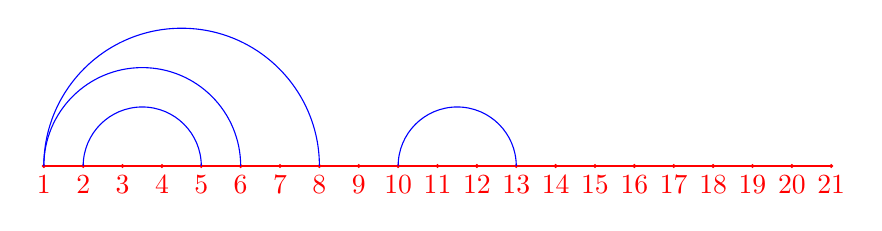
\begin{tikzpicture}[scale=0.5]


\foreach \i in {1,...,20} {
        \draw[red] (\i,1) -- (\i + 1,1)node[pos=0.0,below] {\i};
        \filldraw[red] (\i,1) circle (1pt);


 }

\draw[red] (21,1) -- (20,1)node[pos=0.0,below] {21};
\filldraw[red] (21,1) circle (1pt); 



\draw[blue, thin] (1,1) arc(180:0:3.5); 
\draw[blue, thin] (1,1) arc(180:0:2.5); 
\draw[blue, thin] (2,1) arc(180:0:1.5);
\draw[blue, thin] (10,1) arc(180:0:1.5);
\end{tikzpicture} 
\input{queue1}
\caption{Two Stacks and the queue}
 \label{fig:Two Stacks and the queue}
 \end{figure}

The decomposition theorem is considered an important step in formulating approximation algorithms for contact map overlap of self-avoiding walks. The first result in computing the contact map overlap is a $4$-approximation algorithm. Each walk in such setting is decomposed into two stacks and two staircases of maximum degree $2$. This is because each walk can be decomposed into two stacks and a queue and each queue can be decomposed into two staircases of maximum degree $2$. Polynomial time algorithms for these special cases are used to compute the 4-approximation algorithm. Considering the above decomposition theorem and with some minor modifications, it can further be shown that any contact map of a self-avoiding walk in two dimensional square lattice can be broken into one stack and two augmented staircases. This decomposition theorem is used to formulate the polynomial-time 3-approximation algorithm.

\citet{goip99} also state two very important open problems. One is to find better approximation ratio for contact map overlaps in two-dimensional lattice. The other is to find properties of three-dimensional self-avoiding walks and investigate if any approximation results can be obtained for the same. These two open problems are addressed in \citet{agmw07}. 

\section {Improvement of Result in 2-dimensional model}
\citet{agmw07} address two open problems from \citet{goip99}. Although they do not provide a better approximation algorithm, the running time of the 6-approximation algorithm is $O(n^3 \log n)$ which is a significant improvement from the previous algorithm in two dimensions. The algorithms described in the next two subsections use the same structure of proof from \citet{goip99}.
\subsection{Staircase and CMO}
Towards simplifying the problem of calculating the contact map overlap measure, an algorithm for computing the same between a staircase and the graph of a self-voiding walk is presented in this section. One can observe that if $T=(V,E)$ is a 2-staircase graph then $E$ can be decomposed into two subsets $E_{1}$ and $E_{2}$ in $O(|E|)$ time where $T_{1}=(V,E_{1})$ and $T_{2}=(V,E_{2})$ are 1-staircase graphs. To understand why this is possible at all, one can consider assigning the edges corresponding to each of the degree 2 nodes of the original staircase $T$ to sets
$E_{1}$ and $E_{2}$ alternatively (Fig. \ref{fig:staircasedecompisition} illustrates this formulation). Since a subgraph of a staircase is also a staircase, both $T_{1}$and $T_{2}$, formed by the above process, become degree $1$ staircase graphs. Therefore, to measure the contact map similarity between a 2-staircase graph and a general graph, it is sufficient to propose algorithm for computing contact map measure between a 1-staircase graph and a general graph.

\begin{figure}[htbp]
\begin{minipage}[b]{0.33\linewidth}
\centering
 \input{staircasedecomp}
 \vspace{0.65cm}
\end{minipage}
\begin{minipage}[b]{0.33\linewidth}
\centering
 \input{staircasedecomp1}
 \vspace{0.65cm}
\end{minipage}
\begin{minipage}[b]{0.33\linewidth}
\centering
 
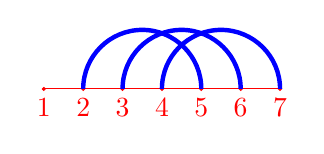
\begin{tikzpicture}[scale=0.5]
\centering
\label{staircasedecompisition}

\foreach \i in {1,...,6} {
        \draw[red] (\i,1) -- (\i + 1,1)node[pos=0.0,below] {\i};
        \filldraw[red] (\i,1) circle (1pt);
 }

\draw[red] (7,1) -- (6,1)node[pos=0.0,below] {7};
\filldraw[red] (7,1) circle (1pt);

\draw[blue, ultra thick] (2,1) arc(180:0:1.5);
\draw[blue, ultra thick] (3,1) arc(180:0:1.5);
\draw[blue, ultra thick] (4,1) arc(180:0:1.5);
\end{tikzpicture}
 \vspace{0.65cm}
\end{minipage}
\caption{A 2-staircase and its decomposition into two 1-staircase}
 \label{fig:staircasedecompisition}
\end{figure}


For further description of the algorithm, the concept of ``cluster" is important which is defined as a set of mutually overlapping edges. From the definition of a staircase graph, it should be obvious that each 1-degree staircase graph consists of only disjoint clusters of edges. Consider one such 1-degree staircase graph $G_1$ consisting of clusters $C_{1}, C_{2}, \cdots, C_{K}$ which is compared to a contact map $G_2=(V_2,E_2)$. Let ${G_1}_{i}$ be the subgraph of $G_1$ consisting of clusters $C_{1}, C_{2}, \cdots, C_{i}$ and ${G_2}_{(1j)}$ be the subgraph of $G_2$ consisting of vertices with indices running from $1$ to $j$ along with the associated edges. A quantity $D(i,j)$ is defined
now to measure the contact map overlap between ${G_1}_{i}$ and ${G_2}_{(1j)}$. The idea is to propose algorithm and measure the complexity for the subgraphs and apply recursion thereafter to compute the similarity measure over the entire graphs.

A consequence of such construction is the following recursive update equation:
\begin{equation}
\label{dim1}
D(i,j) = \max_{0\le r\le m_{i}}\{D(i-1,\Phi(j,r)-1)\} + r,
\end{equation}
where $\Phi(j,r)$ denotes the largest integer $h$ such that ${G_2}_{(hj)}$ contains a cluster of size $r$ as its
subgraph and $m_{i}$ is the number of edges in cluster $C_{i}$.
Let $h^{*}$ denote the largest integer such that ${G_2}_{({h^{*}j})}$ contains $r^{*}$ number of edges obtained from a successful maximal mapping $f^{*}$ between $C_{i}$ and ${G_2}_{({1j})}$. Then, intuitively Eq. \ref{dim1} implies that once one has computed $D(i-1,h^{*}-1)$, the maximum overlap measure between ${G_1}_{(i-1)}$ and ${G_2}_{({(h^{*}-1)j})}$, one can compute $D(i,j)$ by simply solving a maximization problem, assuming $\Phi(j,r)$ is pre-computed. One can see that each step of such recursion takes $O({n_1}_{i})$ time and hence the total computation time is $O(\sum_{{n_1}_{i}}n_2)$ or $O({n_1}{n_2})$.

Pre-computation of $\Phi(j,r)$ can be performed using the following recursive update:
\begin{equation}
\label{rec2}
\Phi(j,r) = \max\{\Phi(j-1,r), \max_{e=(i,j)\in E}\tilde{\Phi}(e,r)\}.
\end{equation}
Here $\tilde{\Phi}(e,r)$ is an auxiliary function corresponding to edge $e\in G_2$ and $r\le {n_2}$ such that $\tilde{\Phi}(e,r)$ is the largest integer $h$ so that ${G_2}_({hj})$ contains a cluster of size $r$ as
its subgraph with $e$ being the rightmost edge of the cluster. Computation of each of such auxiliary functions can be performed in $O({n_2}\log {n_2})$ time according to arguments given in \citet{k73}. Since $G_2$ has $O(n_2)$ edges, total time spent in such computation is $O({n_2}^{2}\log {n_2})$. Combined everything together, the contact map measure between
$G_1$ and $G_2$ can be computed in $O({n_1}{n_2}+{n_2}^{2}\log {n_2})$ time.


\subsection{Stack and CMO}
Similar to the construction of the algorithm in the last section, \citet{agmw07} show that the contact map overlap between a $2$-stack and any two dimensional graph can be constructed in $O({n_1}{n_2}^{2}\log n_1)$ time where $n_1$ is the number of vertices in the $2$-stack and $n_2$ is the number of vertices in the two dimensional graph. To illustrate the same, the stack has been represented as a tree where each node corresponds to an edge of the tree and a node $e^{\prime}$ can be considered as the child node of $e$ when $e$ contains $e^{\prime}$ \citep{agmw07}.

\begin{figure}[htbp]
\begin{minipage}[b]{0.5\linewidth}
\centering
 
\centering
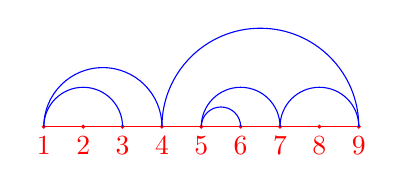
\begin{tikzpicture}[scale=0.5]


\foreach \i in {1,...,8} {
        \draw[red] (\i,1) -- (\i + 1,1)node[pos=0.0,below] {\i};
        \filldraw[red] (\i,1) circle (1pt);


 }

\draw[red] (9,1) -- (8,1)node[pos=0.0,below] {9};
\filldraw[red] (9,1) circle (1pt); 



\draw[blue, thin] (1,1) arc(180:0:1); 
\draw[blue, thin] (1,1) arc(180:0:1.5);
\draw[blue, thin] (4,1) arc(180:0:2.5); 
\draw[blue, thin] (5,1) arc(180:0:0.5); 
\draw[blue, thin] (5,1) arc(180:0:1);
\draw[blue, thin] (7,1) arc(180:0:1);

\end{tikzpicture} 
 \vspace{0.65cm}
\end{minipage}
\begin{minipage}[b]{0.5\linewidth}
\centering
 \includegraphics[width=0.5\textwidth]{tree}
 \vspace{0.65cm}
\end{minipage}
\caption{Stack and its tree representation}
 \label{fig:stacktree}
\end{figure}
The authors show the results for a $1$-stack and any two dimensional graph and then the results are extended to compute the overlap between a $2$-stack and graph. Let
$G_1 = (V_1,E_1)$ be the 1-stack of size $n_1$ and $G_2 = (V_2,E_2)$ a contact map of size $n_2$. Further, let $e \in E_1$ be the rightmost edge in $G_1$ with the highest right end-point and $e^{\prime} \in E_2$ be a similar edge in $G_2$. Since $G_1$ is a 1-stack, $e$ is not contained in any other edge, so $e$ and $e^{\prime}$ must match each other. If $(v_l,v_j)$ be the end points of such an edge $e$ in $G_1$ and $(v_{l^{\prime}},v_{j^{\prime}})$ be the edge of $e^{\prime}$ in $G_2$, then the problem can be divided into two subproblems where $(v_i,v_l)$ and $(v_l,v_j)$ are the starting and ending vertices of the two subgraphs of $G_1$, and $(v_{i^{\prime}},v_{l^{\prime}})$ and $(v_{l^{\prime}},v_{j^{\prime}})$ are the starting and ending vertices of the two subgraphs of $G_2$. Hence, the maximum contact overlap can be computed by the same dynamic programming technique used by \citet{goip99} where at each step the graph is divided into subgraphs with respect to the rightmost edge. Thus the quantity $D(i,j,i^{\prime},j^{\prime})$, the optimal match between $v_i,\cdots,v_j$ and $v^{\prime}_i,\cdots,v^{\prime}_j$, can be given by:
\begin{equation}
\label{scmo1}
D(i,j,i^{\prime},j^{\prime}) = \max\{D(i,j-1,i^{\prime},j^{\prime}),D(i,j,i^{\prime},j^{\prime}-1),(D(i,l-1,i^{\prime},l^{\prime}-1)
+D(l,j-1,l^{\prime},j^{\prime}-1)+1)\},
\end{equation}
where $(v_l,v_j) \in E_1$ and $(v^{\prime}_l,v^{\prime}_j) \in E_2$. The time taken to compute this is $O({n_1}^2{n_2}^2)$. In the equation, the last 1 is when the rightmost edge of each have been mapped. This is known as the ``right matching" algorithm. Similarly the algorithm which matches the left edges is known as the ``left matching" algorithm, the running time of which is still $O({n_2}^4)$. Using a tree decomposition theorem proposed by \citet{klein98}, \citet{agmw07} show that if the process is interleaved, \emph{i.e.} at some points the rightmost edges are matched and at others the leftmost edges are matched thereby meeting in the middle, then the total number of edges that need to be visited is $O({n_1} \log {n_1})$. This is where the tree structure of the stack becomes useful. These edges need to be mapped to all the edges of $V_2$ requiring $O({n_2}^2)$ time. Hence, the total time to compute $D$ is $O({n_1}{n_2}^2\log n_1)$. The vertices which have degree 2 are also handled in the same time bound.

\citet{goip99} show that any two-dimensional contact map can be decomposed into two 2-stacks and two 2-staircase. Further, each 2-staircase can be decomposed into two 1-staircase in linear time. Considering two-dimensional contact maps $G_1$ and $G_2$ of size $n$ each, $G_1$ can be decomposed into six subgraphs and then maximum contact overlap can be calculated between the set of these $6$ subgraphs and $G_2$ rendering a 6-approximation algorithm. The maximum time taken is $O(n^3\log n)$. 

\section {CMO in 3-dimension}
\citep{agmw07} present the first result of computing the contact map overlap between two graphs in the case of $3$-dimensional self-avoiding walks. Let $G = (V,E)$ be any ordered graph with an ordered set of vertices $V = (v_1,v_2,\cdots,v_n)$ and $E$ be the edges arranged in increasing order of their left end-points \emph{i.e.} $E = \{e_1=(v_{s_1},v_{t_1}),\cdots,e_u=(v_{s_u},v_{t_u})\}$, where $s_1 \leq \cdots \leq s_u$ are the starting vertices of the edges. Further, let $\tau = (t_1,\cdots,t_u)$  and $\sigma$ be defined as the smallest integer $k$ such that $\tau$ is decomposed into $k$ monotonically increasing or decreasing subsequences. The decomposition of $\tau$ into $k$ monotonically increasing or decreasing subsequences takes place in $O(n \log n)$ time according to the algorithm suggested in \citet{k73}. Since $G$ is a constant graph of degree $n$, length of $\tau$ is $O(n)$ and the number of iterations to create this subsequence is at most $O(\sqrt n)$ \citep{erd35}.

Let the subsequence extracted at the $k^{\text{th}}$ iteration be given by $\tau _k = (t_{i1},....,t_{il})$ and the subgraph formed by these edges in $\tau _k$ be called $T_k$ where the edge set is given by $E _k =\{(s_{i1},t_{i1}),\cdots,(s_{il},t_{il})\}$. It can be shown that either $T_k$ is a stack (in a decreasing subsequence) or a queue (in an increasing subsequence). Two edges $e_i=(v_{s_i},v_{t_i})$ and $e_j=(v_{s_j},v_{t_j})$ are so taken that $t_i \in \tau _k$ at index $s_i$ and $t_j \in \tau _k$ at index $s_j$. Without loss of generality, for any subsequence one can consider $t_i < t_j$. If $\tau _k$ is an increasing subsequence, $s_i<s_j$ and consequently, $e_i$ does not contain $e_j$ and \emph{vice versa} for which $\tau _k$ becomes a queue. For a decreasing subsequence $s_i >s_j$ and $s_j$, the left index point of $e_j$, is less than $s_i$, the left index point of $e_i$, and $t_j$, the right index point of $e_j$, is more than $t_i$, the right index point of $e_i$. Thus $e_j$ contains $e_i$ and hence $T_k$ is a stack.

Now at any iteration,  $\tau _k$ is either a stack or a queue. Since each queue can be divided into two staircases, the total number of subgraphs is at most $O(\sqrt n)$. Again, since each subgraph is computed in $O(n \log n)$ time and there are $\sigma$ of such subgraphs, the total running time is $O(\sigma n \log n)$.

Analogous to the contact map overlap in  $2$-dimensional walks, to construct the overlap between two contact maps $G_1$ and $G_2$ of two $3$-dimensional walks, either $G_1$ or $G_2$ is decomposed into $\sigma$ stacks and staircases and then contact map overlap of each can be computed in polynomial time. Contact map overlap will be computed between these $\sigma$ subgraphs and $G_2$, achieving a $\sigma$-approximation algorithm. Summing up the running time of matching each of the smaller graphs to the other, the total running time is $O(n^3 \log n)$. 

\chapter{Exact Algorithms for Maximum CMO}
\label{exact}
Though NP-hard problems are not solvable in polynomial time, they can be solved through exhaustive search. It is when the size of the search space grows, the running time becomes astronomically large or memory becomes a bottleneck. However, for some special cases, it is possible to design algorithms that are faster than the exhaustive search. These algorithms are called ``Exact" algorithms. There exists four such exact algorithms for the maximum CMO problem where the branch-and-bound framework is adopted to ensure global optimality. The four algorithms are -- B \& Cut \citep{carr00}, Clique \citep{strick05}, LAGR \citep{cap04} and CMOS \citep{xie07}. The algorithm proposed by \citet{anmy11} and discussed extensively in this report outperforms the other exact algorithms and successfully reproduces the results of previous algorithms in much less time. The sections below discuss the formulation of the mathematical model and also the structure and proofs of the algorithm in \citet{anmy11}.

\section {Integer Programming Model for CMO}
The framework proposed by \citet{anmy11} represents the CMO problem as an integer programming problem.
When tested on a widely used benchmark, the Skolnick set \citep{gosk94}, the proposed algorithms for solving the optimization problem outperforms other existing exact algorithms both in terms of time efficiency and quality of bounds. To describe the formulation further, let us consider the contact maps of two proteins $P_1$ and $P_2$ given by $G_1 = (V_1,E_1)$ and $G_2 = (V_2,E_2)$, where $n_1$ is the number of vertices in $G_1$ and $n_2$ is the number of vertices in $G_2$. For convenience, contact maps of both the proteins will be represented by the index $m$ that takes value $1$ for $P_1$ and value $2$ for $P_2$. The right and left neighbour of any vertex $i$ in the $m^{\text{th}}$ protein is given by $\delta_m^+ = \{j | j>i ,(i,j) \in E_m)\}$ and  $\delta_m^- = \{j | j<i ,(j,i) \in E_m)\}$ respectively. For every edge $(i,j)\in E_1$ mapped to  $(k,l)\in E_2$, a non-crossing alignment happens when $i<j$ and $k<l$. Feasible alignments of two proteins $P_1$ and $P_2$ are given by non-crossing matchings in the complete bipartite graph $B$ with a vertex set $V_1\cup V_2$.
For every such non-crossing alignment, a weight $w_{ikjl}$ is introduced according to the following rule:
\begin{equation}
\label{rec11}
w_{ikjl}=\begin{cases}
    1, & \text{ if } (i,j) \in E_1 \text{ and } (k,l) \in E_2,\\
    0, & \text{ otherwise}.
  \end{cases}
\end{equation}
If $M$ represents the complete set of non-crossing matching in $B$, then $w(M)$ is the sum of all the weights over edges in $M$ and the CMO problem is nothing other than maximizing $w(M)$.

\begin{figure}[ht]
\centering
 \includegraphics[width=0.7\textwidth]{pic1}
 \caption{Bipartite and Grid Graph Representation}
 \label{fig:Bipartite and Grid Graph Representation}
\end{figure}

Now, let us consider an interesting transformation of the problem also studied extensively in \citet{andonov04, andonov08}. The edges of $B$ are mapped onto a gird of size $n_1\times n_2$ which is denoted by $B^{\prime} = (V^{\prime},E^{\prime})$. The mapping abides by the following rule -- a vertex $(i,k) \in V^{\prime}$ if there exists an edge $(i,k)$ in $B$ and an arc $(i,k)(j,l) \in E^{\prime}$ if $w_{ikjl} = 1$. A bipartite graph $B$ and its corresponding grid graph transformation are illustrated in Fig. \ref{fig:Bipartite and Grid Graph Representation} \citep{anmy11}. In Fig. \ref{fig:Bipartite and Grid Graph Representation}, only the edges of the considered matching are shown. Further, let's consider ``feasible path" in this grid which is defined as an arbitrary sequence of vertices whose coordinates are arranged in increasing order. For example, in Fig. \ref{fig:Bipartite and Grid Graph Representation}, a feasible path is a path connecting the vertices $(1,1)$, $(2,3)$, $(3,4)$ and $(5,5)$.
Since, $M = \{(1,1)(2,3),(3,4)(5,5)\}$, according to the update rule given in Eq. \ref{rec11}, $w(M) =2$. One can 
see that the arcs $(1,1)(2,3)$ and $(3,4)(5,5)$ are activated only in Fig. \ref{fig:Bipartite and Grid Graph Representation} which contribute towards making $w(M)=2$. Therefore, in the transformed representation $B^{\prime}$, one can see that the objective is to maximize the number of such arcs whose vertex set forms the feasible path.

By assigning a binary variable $x_{ik}$ to each vertex $(i,k)\in B^\prime$ and a binary variable $y_{ikjl}$ to each arc $(i,k)(j,l)\in B^\prime$ and considering $X$ to be a feasible path in $B^\prime$, the maximum CMO problem can be represented as an integer programming problem as follows:
\begin{equation}
\label{rec1}
v(\mathbf{x},\mathbf{y}) = \max_{\mathbf{x},\mathbf{y}} \sum\limits_{(ik)(jl) \in E^{\prime}} y_{ikjl} \text{, subject to,}
\end{equation}
\begin{equation}
\label{rec2}
x_{ik}  \geq \sum\limits_{l \in \delta _2 ^+(k)}  y_{ikjl} ,	    j\in {\delta _1^+(i)}, i \in [1,n_1-1] , k \in [1,n_2-1],
\end{equation}
\begin{equation}
\label{rec3}
x_{ik}  \geq \sum\limits_{l \in \delta _2 ^-(k)}  y_{ikjl} ,	    j\in {\delta _1^-(i)}, i \in [2,n_1] , k \in [2,n_2],
\end{equation}
\begin{equation}
\label{rec4}
x_{ik}  \geq \sum\limits_{l \in \delta _1 ^+(i)}  y_{ikjl} ,	    l\in {\delta _2^+(k)}, i \in [1,n_1-1] , k \in [1,n_2-1],
\end{equation}
\begin{equation}
\label{rec5}
x_{ik}  \geq \sum\limits_{j \in \delta _2 ^-(i)}  y_{ikjl} ,	    l\in {\delta _2^-(k)}, i \in [2,n_1] , k \in [2,n_2],
\end{equation}
\begin{equation}
\label{rec6}
\{x_{ik}\} \in X,
\end{equation}
\begin{equation}
\label{rec7}
\sum\limits_{l=1}^k  x_{il} + \sum\limits_{j=1}^{i-1}  x_{jk} \leq 1  ,          i \in [1,n_1], k \in [1, n_2].
\end{equation}
Here, $\mathbf{x} = \{x_{ik}\}$ and $\mathbf{y} = \{y_{ikjl}\}$. A feasible path $X$ is constructed by taking a complete grid graph and then pruning the edges based on the constraints described above. To understand the first constraint (Eq. \ref{rec2}) in details, let us consider a CMO problem where the $i^{\text{th}}$ residue from one protein is mapped to the $k^{\text{th}}$ residue of the other protein. Considering that $(i,j)\in E_{1}$ and the fact that CMO is an order preserving bijection, $j$ can only be mapped to one point in the the second contact map \emph{i.e.}, $l$ in the second contact map will be unique. Constraint \ref{rec4} is similar to the constraint \ref{rec2} but corresponds to the reverse order. If there is an edge from $k$ to $i$ in the bipartite graph (\emph{i.e} $k^{\text{th}}$ residue from the second protein is mapped to $i^{\text{th}}$ residue in protein 1 )and if $(k,l)\in E_{2}$ is an edge in the second contact map, then $j$(the point $l$ can be mapped to) of the first contact map should also be unique. Here the summation signifies that for all values of $l$, only one can be 1,the remaining has to be 0. Similarly constraints \ref{rec4} and \ref{rec5} are constructed. The sets of the right and left neighbours are useful to formulate the same. Again weight $w_{ikjl}$ is one when the matching is non crossing, so the arc $(i,k)(j,l)$ is activated i.e. $y_{ikjl} = 1$ iff $x_{ik} = 1$ and $x_{jl} = 1$.

Constraint \ref{rec7} can be understood with the following example. Let $i$ be any residue in $P_1$. Now if $i$ is mapped to $k$ in $P_2$,then $x_{ik}$ is $1$ and it satisfies the constraint. If $i$ is not mapped to $k$, then either $i$ will be mapped to any element from $1$ to $(k-1)$ or $k$ will be mapped to any element from $1$ to $(i-1)$. This also reiterates the fact that there is only one bijective mapping between a residue in one protein to the other in another protein. Again, this mapping should be non-crossing, thereby reassuring order-preserving bijection.

\section {Solution of Integer Programming Model for CMO}
The objective function in Eq. \ref{rec1} can be optimized using different techniques. Earlier approaches
\citep{carr00,cap04} solve the problem using only branch-and-bound technique \citep{past82,bets97} or branch-and-cut technique the latter of which can be considered as an \emph{integer constrained relaxation} method for integer programming \citep{mitc98}. However, as suggested in the optimization literature \citep{bert99,bets97}, significant computation advantage can be gained by performing \emph{Lagrangian relaxation} as well. In such relaxation, first a feasible set is formulated where the \emph{Lagrangian} is optimized \emph{w.r.t} the \emph{primal variables} and the dual objective is optimized thereafter yielding a lower (for minimization) or upper bound (for maximization) to the original objective. The duality gap can further be improved by proposing better constraint sets \citep{bert99,bets97}. Additionally, in case of a non-zero duality gap, one can employ branch-and-bound algorithm on the smaller feasible set obtained from the Lagrangian relaxation. In this section, first a tighter constrain set, proposed by \citet{anmy11}, is presented which is then followed by the Lagrangian relaxation and an application of the branch-and-bound algorithm.

\subsection{Finding a Tighter Constrain Set}

Tightening the solution space may improve the bound of the proposed Lagrangian \citep{ackm05,bert99}. To increase the constrain set for a tighter relaxation, the constraint \ref{rec3} and \ref{rec5} are replaced by the following two constraints:
\begin{equation}
\label{rec8}
x_{ik}  \geq \sum\limits_{(r,s) \in row _{ik}(j)}  y_{rsik} ,	    j\in {\delta _1^+(i)}, i \in [1,n_1] , k \in [1,n_2]
\end{equation}
\begin{equation}
\label{rec9}
x_{ik}  \geq \sum\limits_{(r,s) \in col _{ik} (l)}  y_{ikjl} ,	    l\in {\delta _2^-(k)}, i \in [2,n_1] , k \in [2,n_2]
\end{equation}
The construction of $row _{ik}(j)$ and $col _{ik} (l)$ in Eqs. \ref{rec8} and \ref{rec9} can be explained with the Fig. \ref{fig:Construction of tighter constraint set}. The grey area in each of the images is the rectangle formed by $\delta_1^-(i)$ rows and $\delta_2^-(k)$ colums for any vertex (i,k) in the graph. Let $(i_1,i_2,\cdots,i_s)$ and $(k_1,k_2,\cdots,k_t)$ be the ordered set of vertices in $\delta_1^-(i)$ and $\delta_2^-(k)$. Considering the vertices in the $l^{\text{th}}$ column to be the pairwise crossing matching, at most one of the points in the vertices of the column will satisfy Eq. \ref{rec5}. The solution remains the same even if the following sets are added to the vertices in the $l^{\text{th}}$ column:$(i_s,k_1),(i_s,k_2),\cdots,(i_s,k_{l-1})$ and $(i_1,k_{l+1},i_1,k_{l+2},\cdots,i_1,k_t)$. The union of these three sets constructs $col _{ik} (l)$. $row _{ik}(j)$ is constructed in a similar fashion.

\begin{figure}[ht]
\centering
 \includegraphics[width=0.7\textwidth]{pic2}
 \caption{Construction of tighter constraint set}
 \label{fig:Construction of tighter constraint set}
\end{figure}

\subsection{Lagrangian Relaxation}
The Lagrangian of the problem in Eq. \ref{rec1} is formed as follows:
\begin{equation}
\label{lagrangian}
\mathcal{L}(\mathbf{x},\mathbf{y},\boldsymbol{\lambda}) = \sum\limits_{(ik)(jl) \in E^{\prime}} y_{ikjl}
+ \displaystyle\sum_{i,k,j\in\delta_{1}^{-1}(i)}\lambda_{ikj}^{h} \left(x_{ik} - \displaystyle\sum_{(r,s)\in\text{row}_{ik}(j)}y_{rsik}\right)
\end{equation}
\begin{equation}
+ \displaystyle\sum_{i,k,l\in\delta_{2}^{-1}(k)}\lambda_{ikl}^{v} \left(x_{ik} - \displaystyle\sum_{(r,s)\in\text{col}_{ik}(j)}y_{rsik}\right)
\end{equation}
with the constraints \ref{rec2},\ref{rec4},\ref{rec6},\ref{rec7} and $\boldsymbol{\lambda} = \{\{\lambda_{ikj}^{h}\}, \{\lambda_{ikl}^{v}\}\}\ge \mathbf{0}$. The maximization over the primal variables
$\mathbf{x},\mathbf{y}$ can be performed in $O(|V^{\prime}|+|E^{\prime}|)$ time and this becomes obvious if the objective in Eq. \ref{lagrangian} is observed more carefully. One can see that the objective decomposes over the primal variables and essentially there are as many subproblems as there are number of primal variables in the objective, each of which can be solved independently. Moreover, two different sets of sub-problems can be defined. The first one corresponds to finding the set of best \emph{local variable} $y_{ijkl}$ pertaining to each vertex $(i,k)\in V^{\prime}$ that respects the constrains. The second one corresponds to finding the best values of the set of \emph{global variables} $\{x_{ik}\}$'s. Simple dynamic programming based computation shows a run time complexity of
$O(|V^{\prime}|+|E^{\prime}|)$.

\begin{figure}[htbp]
\centering
 \includegraphics[width=0.7\textwidth]{pic3}
 \caption{Branch-and-bound Splitting Strategy}
 \label{fig:BB}
\end{figure}

A dual objective function $\mu(\boldsymbol{\lambda})$ is obtained afterwards
by maximizing \ref{lagrangian} over the primal variables. The dual objective, however, has plenty of variables $\boldsymbol{\lambda}$ and hence sub-gradient descent \citep{hewc74,duhs11} with adaptive step-size regulation is used. However, the bound so obtained is not tight and there might exist duality gap either because of problem formulation or from the approximations used in the sub-gradient optimization. To make the solution even better, branch-and-bound algorithm is used as discussed in the next section.

\subsection{Branch-and-bound Algorithm}

A branch-and-bound algorithm works by enumerating over all possible solution sets and maintaining a tree structure to prune the search space based on the value of the objective function. Parts of the tree where the objective function takes bigger value (in case of maximization), are preferred over other parts of the tree.
A node in the tree in the current setting is given by by $n_2$ couples $(b_k, t_k)$ for $k_2 \in [1, n2]$ which define the candidate vertex set $Cand$ (the white area in-between the two broken lines on Fig. \ref{fig:BB}).
A vertex $(j, l)$ of the graph $B^{\prime}$ belongs to $Cand$ if $b_l\leq j \leq t_l$.
For any vertex $(j,l) \in Cand$, two sets are created:
$U(j,l)= \{(i, k) \in Cand : (i, k)=(j, l), i\ge j, k\le l\}$
and $D(j,l) = f(i, k) \in Cand : i\le j, k\ge l\}$.
By definition, if a feasible path has a vertex in $U(j,l)$, it cannot
have one in $D(j,l)$, and \emph{vice versa}.
Let $(rbest, cbest)$ be the $\arg\max_{(j, l)\in Cand} \min (\|D(j, l)\|, \|U(j, l)\|)$. Now, the two descendants of the current node are obtained by discarding from its feasible set the vertices belonging to the two respective domains $U(rbest,cbest)$ and $D(rbest, cbest)$ (refer to Fig. \ref{fig:BB}). The goal of this strategy is twofold: to create descendants that are balanced in sense of feasible set size and to reduce maximally the parent node’s feasible set. 


